\section{What Is Simulation?}

Astronomy is an observational science.  Unlike in terrestrial physics,
we do not have the luxury of being able to build a model system and do
physical experimentation on it to understand the core physics.  We
have to take what nature gives us.  Simulation enables us to build a
model of a system and allows us to do virtual experiments to
understand how this system reacts to a range of conditions and
assumptions.

It's tempting to think that one can download a simulation code, set a
few parameters, maybe edit some initial conditions, run, and then have
a virtual realization of some astrophysical system that you are
interested in.  Just like that.  In practice, it is not this simple.
All simulation codes make approximations---these start even before one
turns to the computer, simply by making a choice of what equations are
to be solved.  Typically, we have a system of PDEs, and we need to
convert the continuous functional form of our system into a discrete
form that can be represented in the finite memory of a computer.  This
introduces yet more approximation.

%V\&V

Blindly trusting the numbers that come out of the code is a recipe
for disaster.  You don't stop being a physicist the moment you execute
the code---you job as a computational scientist is to make sure that
the code is producing reasonable results, by testing it against known
problems and your physical intuition.  

Simulations should be used to gain insight and provide a physical
understanding.  
Because the systems we solve are so nonlinear, small changes in the
code or the programming environment (compilers, optimization, etc.)
can produce large differences in the numbers coming out of the code.
That's not a reason to panic.
As such its best not to obsess about precise numbers, but rather the
trends.  To really understand the limits of your simulations, you
should do parameter and convergence studies.

There is no ``\"uber-code''.  Every algorithm begins with approximations
and has limitations.  Comparisons between different codes are
important and common in our field, and build confidence in the
results that we are on the right track.

To really understand your simulations, you need to know what the code
your are using is doing under the hood.  This means understanding the 
core methods used in our field.  These notes are designed to provide
a basic tour of some of the more popular methods, referring to the 
key papers for full derivations and details.  A companion python code,
{\sf pyro} is available to help. 


\section{Numerical Basics}

We assume a familiarity with basic numerical methods, which we
summarize below.  Any book on numerical methods can provide a
deeper discussion of these methods.

\subsection{Sources of Error}

With any algorithm, there are two sources of error we are concerned
with: {\em roundoff error} and {\em truncation error}.  

Roundoff arises from the error inherent in representing a floating
point number with a finite number of bits in the computer memory.  An
excellent introduction to the details of how computers represent
numbers is provided in \cite{goldberg:1991}.  

\begin{exercise}[Machine epsilon]
To see roundoff error in action, write a program to find the value
of $\epsilon$ for which $1 + \epsilon = 1$.  This value of $\epsilon$
is called {\em machine epsilon}.  You will get a different value for
single- vs.\ double-precision floating point arithmetic.
\end{exercise}

Some reorganization of algorithms can help minimize roundoff,
e.g.\ avoiding the subtraction of two very large numbers by factoring as:
\begin{equation}
x^3 - y^3 = (x - y)(x^2 + xy + y^2) \enskip ,
\end{equation}
but roundoff error will always be present at some level.

Truncation error is a feature of an algorithm---we typically
approximate an operator or function by expanding about some small
quantity.  When we throw away higher-order terms, we are truncating
our expression, and introducing an error in the representation.  If
the quantity we expand about truely is small, then the error is small.
A simple example is to consider the Taylor series representation of
$\sin(x)$:
\begin{equation}
\sin(x) = \sum_{n=1}^\infty (-1)^{n-1} \frac{x^{2n-1}}{(2n-1)!} 
\end{equation}
For $|x| \ll 1$, we can approximate this as:
\begin{equation}
\sin(x) \approx x - \frac{x^3}{6}
\end{equation}
in this case, our truncation error has the leading term $\propto x^5$,
and we say that our approximation is $\mathcal{O}(x^5)$, or
$5^\mathrm{th}$-order accurate.

\begin{exercise}[Convergence and order-of-accuracy]
We will be concerned with the order-of-accuracy of our methods, and a
good way to test whether our method is behaving properly is to perform
a convergence test.  Consider our $5^\mathrm{th}$-order accurate
approximation to $\sin(x)$ above.  Pick a range of $x$'s ($< 1$), and
compute the error in our approximation as $\epsilon \equiv \sin(x) - [
  x - x^3/6 ]$, and show that as you cut $x$ in half, $\epsilon$
reduces by $2^5$---demonstrating $5^\mathrm{th}$-order accuracy.
\end{exercise}

This demonstration of measuring the error as we vary the size
of our small parameter is an example of a {\em convergence test}.

\subsection{Differentiation and Integration}

For both differentiation and integration, there are two cases we might
encounter.  In the first, we have function values, $f_0$, $f_1$,
$\ldots$, at a discrete number of points, $x_0$, $x_1$, $\ldots$, and
we want to compute the derivative at a point or integration over a
range of points.  The second case is when we know a function
analytically and we want to construct a derivative or integral of this
function numerically.  In these notes, we'll be concerned only with
the first case.

\subsection{Differentiation}
\label{ch:intro:diff}
Consider a collection of equally spaced points, labelled with an index
$i$, with the physical spacing between them denoted $\Delta x$.  We
can express the first derivative of a quantity $a$ at 
$i$ as:
\begin{equation}
\left . \frac{\partial a}{\partial x} \right |_i \approx \frac{a_i - a_{i-1}}{\Delta x}
\end{equation}
or
\begin{equation}
\left . \frac{\partial a}{\partial x} \right |_i \approx \frac{a_{i+1} - a_i}{\Delta x}
\end{equation}
%
(Indeed, as $\Delta x \rightarrow 0$, this is the definition of a derivative from calculus.)
Both of these are {\em one-sided differences}.  By Taylor expanding the data
about $x_i$, we see
\begin{equation}
a_{i+1} = a_i + \Delta x \left . \frac{\partial a}{\partial x} \right |_i + \frac{1}{2} \Delta x^2 \left . \frac{\partial^2 a}{\partial x^2} \right |_i + \ldots
\end{equation}
Solving for ${\partial a}/{\partial x} |_i$, we see
\begin{equation}
\left . \frac{\partial a}{\partial x} \right |_i = \frac{a_i - a_{i-1}}{\Delta x} + \mathcal{O}(\Delta x)
\end{equation}
where $\mathcal{O}(\Delta x)$ indicates that the order of accuracy of
this approximation is $\sim \Delta x$.  We say that this is {\em first
  order accurate}.  This means that we are neglecting terms that scale
as $\Delta x$.  This is our truncation error (just as discussed above,
arising because our numerical approximation throws away higher order
terms).  The approximation ${\partial a}/{\partial x} |_i = ({a_{i+1}
  - a_i})/{\Delta x}$ has the same order of accuracy.

\begin{exercise}[Trunction error]
{Show that a centered difference, ${\partial a}/
  {\partial x} |_i = ({a_{i+1} - a_{i-1}})/({2 \Delta x})$, is second order
accurate, i.e.\ its truncation error is $\mathcal{O}(\Delta x^2)$.}
\end{exercise}

% this figure was created by figures/intro/derivatives.py
\begin{figure}[t]
\centering
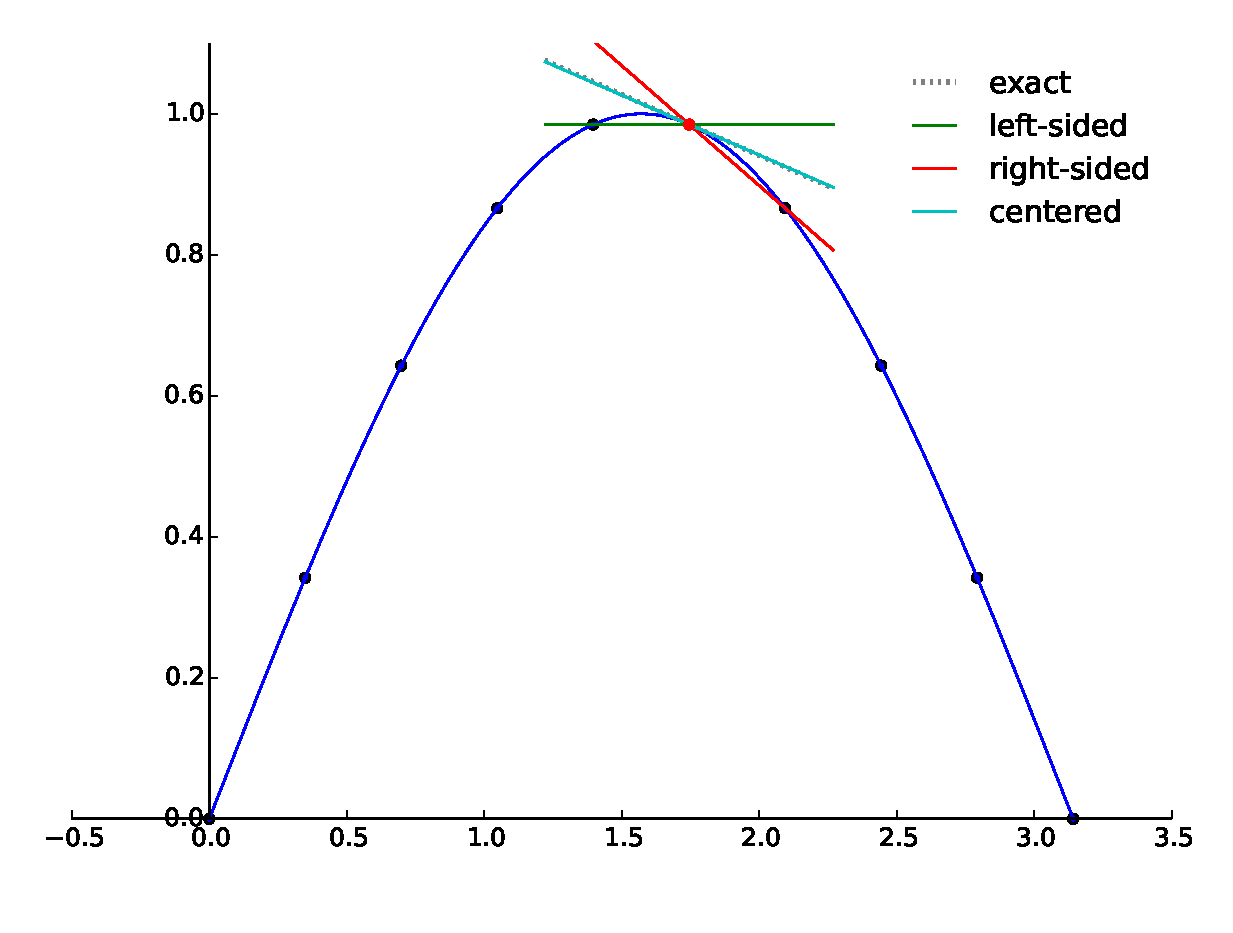
\includegraphics[width=0.8\linewidth]{derivs}
\caption{\label{fig:derivs} A comparison of one-sided and centered
difference approximations to the derivative of $\sin(x)$.}
\end{figure}

Figure~\ref{fig:derivs} shows the left- and right-sided first-order
differences and the central difference as approximations to
$\sin(x)$. Generally speaking, higher-order methods have lower
numerical error associated with them, and also involve a wider range
of data points.

An alternate scenario is when you know the analytic form of the
function, $f(x)$, and are free to choose the points where you evaluate
it.  Here you can pick a $\delta x$ and evaluate the derivative as
\begin{equation}
\frac{df}{dx} = \frac{f(x+\delta x) - f(x)}{\delta x}
\end{equation}
An optimal value for $\delta x$ requires a balance of truncation error
(which wants a small $\delta x$)  and roundoff error (which becomes large
when $\delta x$ is close to machine $\epsilon$).  A nice discussion of
this is given in \cite{yak}.  Comparing the result with different choices
of $\delta x$ allows for error estimation and an improvement of the result
by combining the results with $\delta x$ and $\delta x/2$ (this is the
basis for a method called {\em Richardson extrapolation}.

Second- and higher-order derivatives can be constructed in the same fashion.


\subsection{Integration}

Midpoint rule

Trapezoid rule

Simpsons rule (exercise, derive Simpson's rule by fitting to a parabola)

compound integration

As with differentiation, if you are free to pick the points where you
evaluate $f(x)$, you can get a much higher-order accurate result.
{\em Gaussian quadrature} is a very powerful technique that uses the
zeros of different polynomials as the evaluation points for the
function to give extremely accurate results.  See the text by
Garcia~\cite{garcia} for a nice introduction to these methods.


\subsection{Root Finding}

The most popular method for root finding is the {\em Newton-Raphson method}.
This arises from a Taylor expansion.  If you wish to find $x$, such that
$f(x) = 0$, and start with an initial guess $x_0$ that you believe is
close to the root, then you can improve the guess to the root by an amount
$\delta x$ as:
\begin{equation}
f(x_0 + \delta x) \sim f(x_0) + f^\prime(x_0) \delta x + \ldots = 0
\end{equation}
Keeping only to $\mathcal{O}(\delta x)$, 
\begin{equation}
\delta x = -\frac{f(x_0)}{f^\prime(x_0)}
\end{equation}
This can be used to correct out guess as $x_0 \leftarrow x_0 + \delta
x$, and we can iterate on this procedure until $\delta x$ falls below
some tolerance.

The main `gotya' with this technique is that you need a good initial guess.
In the Taylor expansion, we threw away the $\delta x^2$ term, but if our
guess was far from the root, this (and higher-order) term may not be small.
Obviously, the derivative must be non-zero in the region around the 
root that you search.

The {\em secant method} for root finding is essentially
Newton-Raphson, but instead of using an analytic derivative,
$f^\prime$ is estimated as a numerical difference.

Many other root finding methods exist, including bisection, which
iteratively halves an interval known to contain a root by looking for
the change in sign of the funciton $f(x)$.

\subsection{ODEs}

Consider a system 
\begin{equation}
\dot{y}_k = f(t, y_k(t))
\end{equation}
Broadly speaking, methods for integrating ODEs can be broken down into
explicit and implicit methods.  Explicit methods difference the system
to form an update that uses only the current (and perhaps previous)
values of the dependent variables in evaluating $f$.  For example, a
first-order explicit update ({\em Euler's method}) appears as:
\begin{equation}
y^{n+1}_k = y^n_k + \Delta t f(t^n, y^n_k)
\end{equation}
where $\Delta t$ is the stepsize. 

Implicit methods different the system in a way that includes the new
value of the dependent variables in the evaluation of $f$---the resulting
implicit system is usually solved using, for example, Newton-Raphson iteration
A first-order implicit update (called {\em backward Euler}) is:
\begin{equation}
y^{n+1}_k = y^n_k + \Delta t f(t^{n+1}, y^{n+1}_k)
\end{equation}

Explicit methods are easier to program and run faster (for a given $
\Delta t$), but implicit methods work better for {\em stiff} problems~\cite{byrnehindmarsh}.

Perhaps the most popular explicit method for ODEs is the 4th-order
Runge-Kutta method (RK4).  This is a multistep method where several
extrapolations to the midpoint and endpoint of the interval are
made to estimate slopes and then a weighted average of these slopes
are used to advance the solution.  The overall procedure looks like:
\begin{equation}
y_k^{n+1} = y_k^n + \frac{\Delta t}{6} (k_1 + 2 k_2 + 2 k_3 + k_4)
\end{equation}
where the slopes are:
\begin{align}
k_1 &= f(t^n, y_k^n) \\
k_2 &= f(t^n + \tfrac{\Delta t}{2}, y_k^n + \tfrac{\Delta t}{2} k_1) \\
k_3 &= f(t^n + \tfrac{\Delta t}{2}, y_k^n + \tfrac{\Delta t}{2} k_2) \\
k_4 &= f(t^n + \Delta t, y_k^n + \Delta t k_3)
\end{align}
This is fourth-order accurate overall.

\begin{figure}[t]
\centering
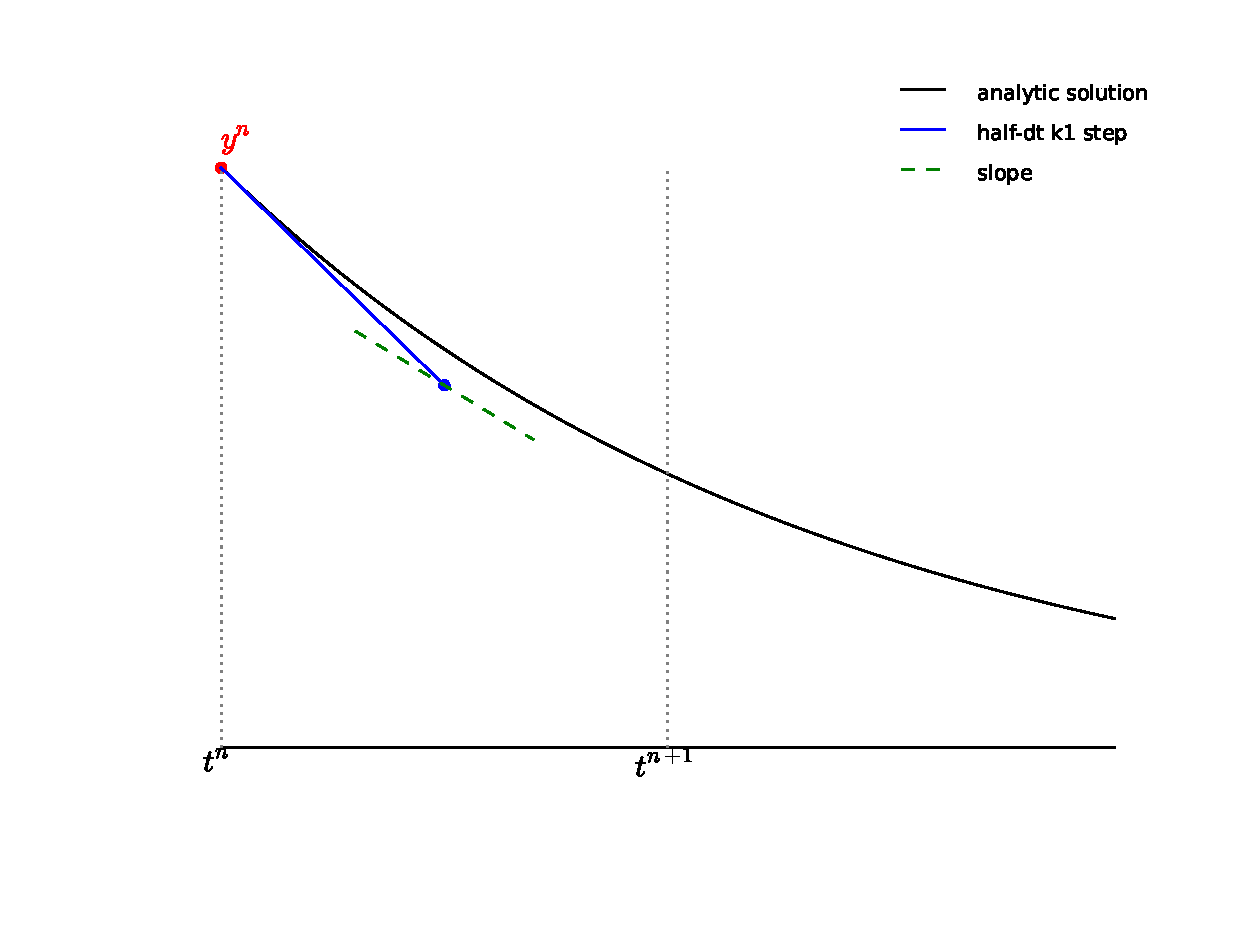
\includegraphics[width=0.65\linewidth]{rk4_k1.eps} \\
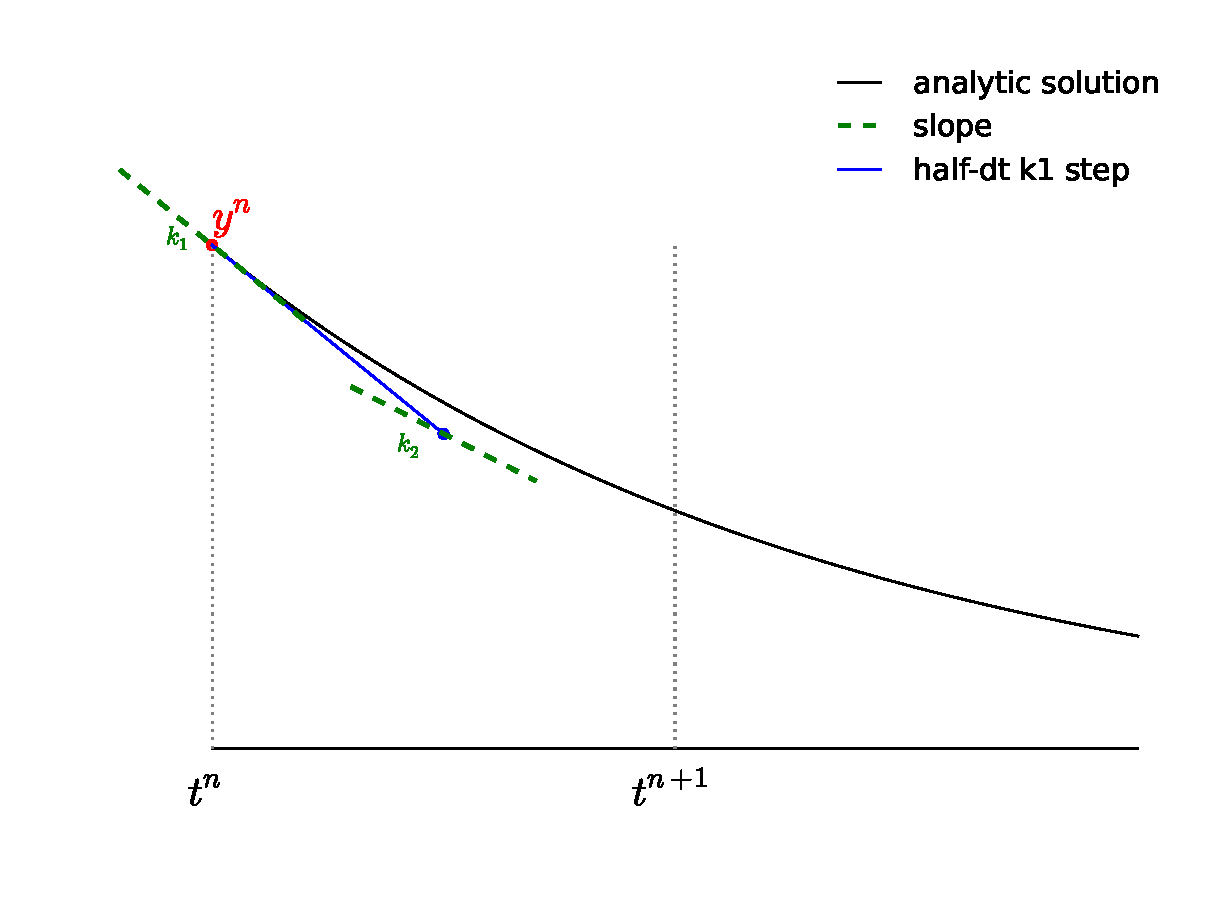
\includegraphics[width=0.65\linewidth]{rk4_k2.eps} \\
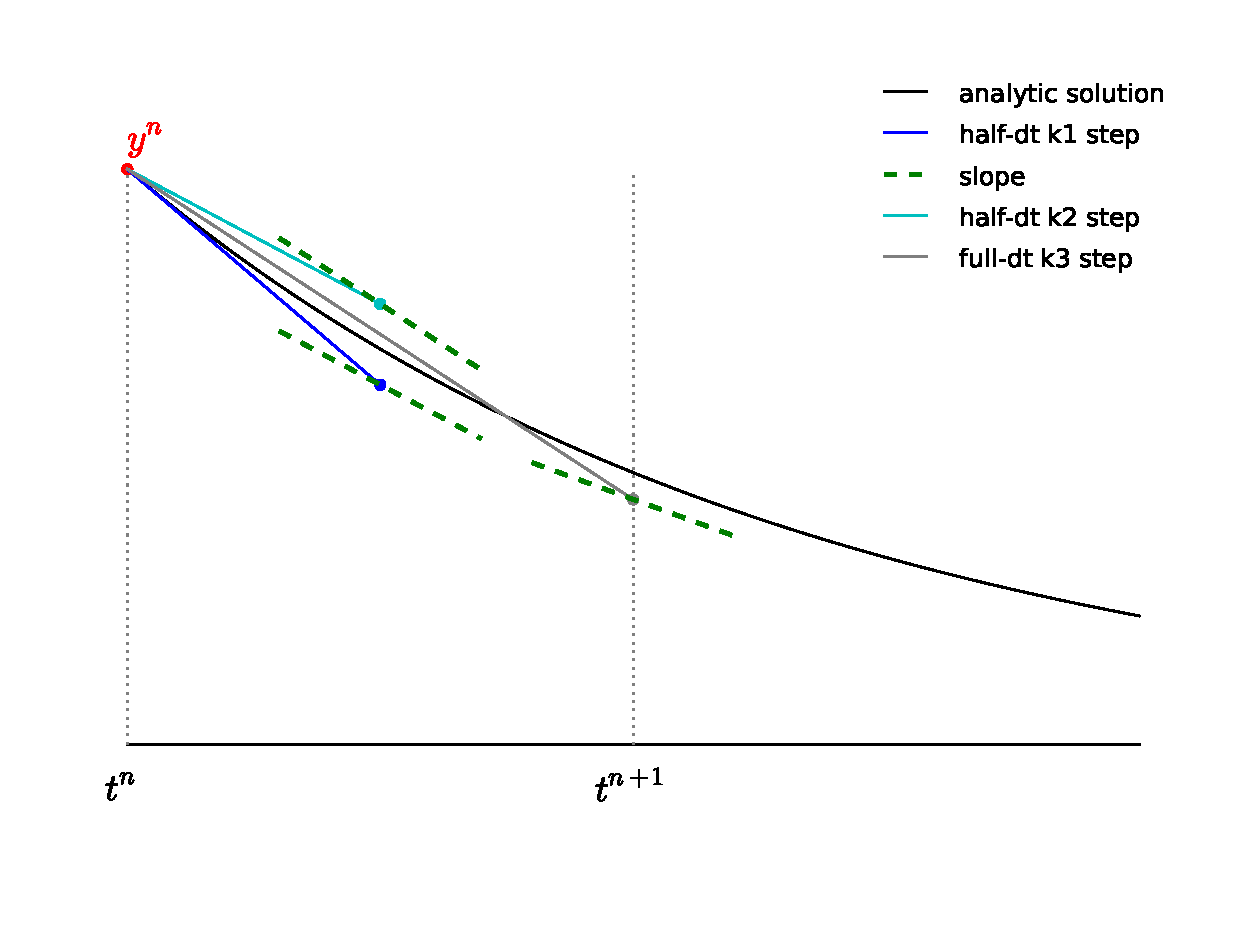
\includegraphics[width=0.65\linewidth]{rk4_k3.eps} \\
%
\caption[The $4^\mathrm{th}$-order Runge-Kutta method] {\label{fig:rk}
  A graphical illustration of the four steps in the
  $4^\mathrm{th}$-order Runge-Kutta method.}
\end{figure}

\begin{figure}[t]
\ContinuedFloat
\centering
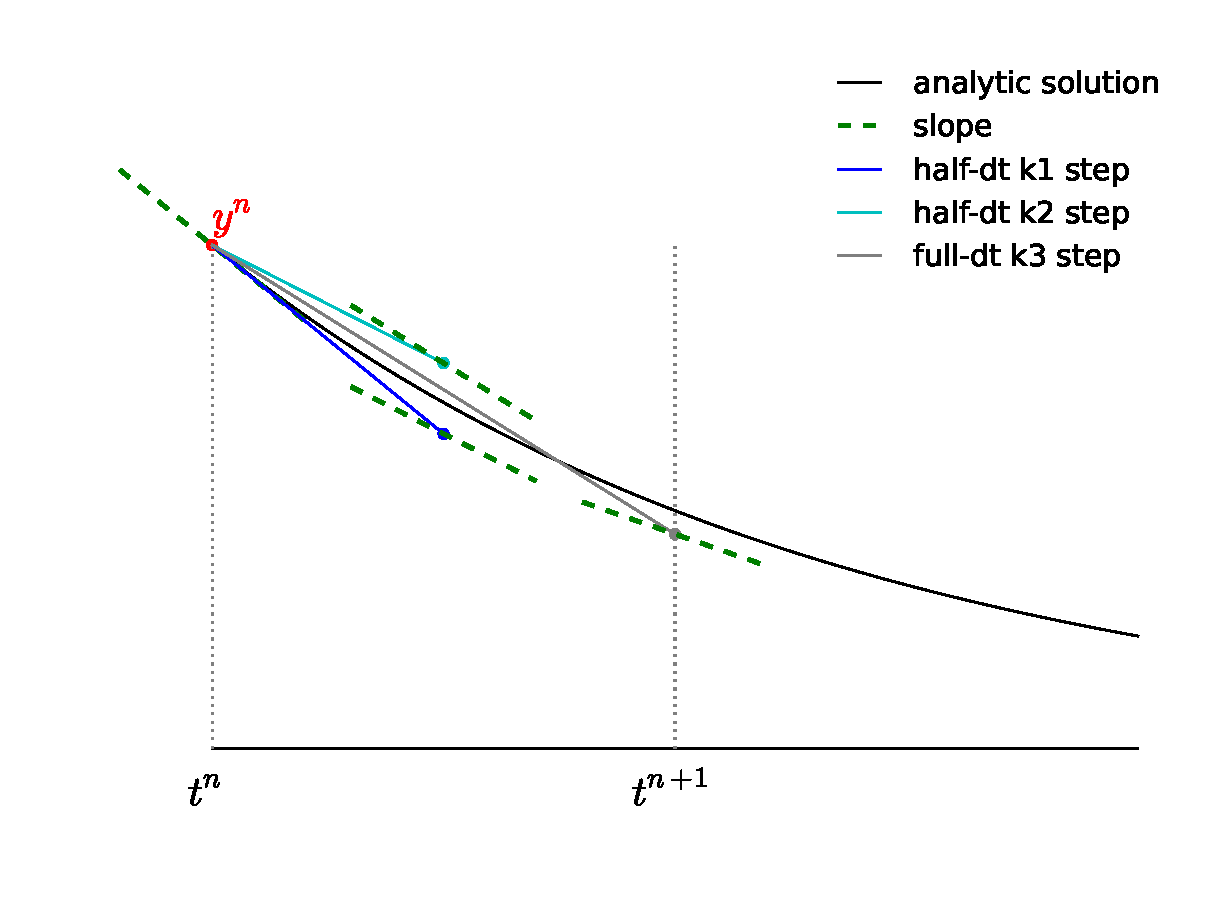
\includegraphics[width=0.65\linewidth]{rk4_k4.eps} \\
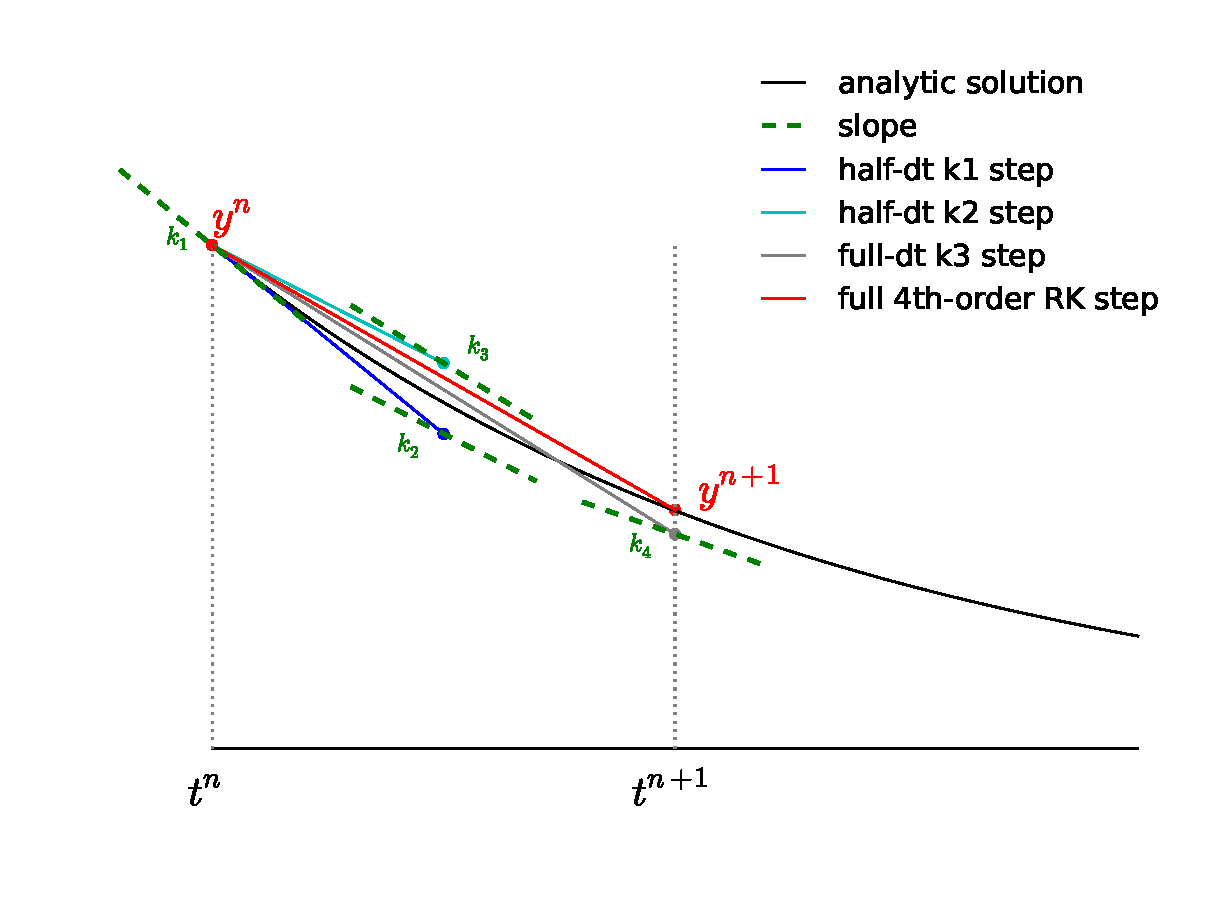
\includegraphics[width=0.7\linewidth]{rk4_final.eps} \\
%
\caption[The $4^\mathrm{th}$-order Runge-Kutta method] {\label{fig:rk}
  (continued) A graphical illustration of the four steps in the
  $4^\mathrm{th}$-order Runge-Kutta method.}
\end{figure}

\begin{exercise}[ODE accuracy]
Consider the orbit of Earth around the Sun.  If we work in the units
of astronomical units, years, and solar masses, then Newton's gravitational
constant and the solar mass together are simply $G M = 4\pi^2$.  We 
can write the ODE system describing the motion of Earth as:
\begin{align}
\dot{\bf x} &= {\bf v} \\
\dot{\bf v} &= -\frac{G M {\bf r}}{r^3}
\end{align}

Integrate this system with the first-order Euler and the RK4 method
and measure the convergence by integrating at a number of different $\Delta t$s.
\end{exercise}

%% \section{A Sample of Public Codes}

%% There are a large number of freely-available codes for modeling astrophysical
%% flows.
